\documentclass[preprint]{elsarticle}

%\usepackage{lineno,hyperref}
%\modulolinenumbers[5]
\usepackage{siunitx}
%\usepackage{doi}
%\usepackage{uri}
%\usepackage{svg}
\usepackage{booktabs}

\journal{Artificial Intelligence in Medicine}

%%%%%%%%%%%%%%%%%%%%%%%
%% Elsevier bibliography styles
%%%%%%%%%%%%%%%%%%%%%%%
%% To change the style, put a % in front of the second line of the current style and
%% remove the % from the second line of the style you would like to use.
%%%%%%%%%%%%%%%%%%%%%%%

%% Numbered
%\bibliographystyle{model1-num-names}

%% Numbered without titles
%\bibliographystyle{model1a-num-names}

%% Harvard
%\bibliographystyle{model2-names.bst}\biboptions{authoryear}

%% Vancouver numbered
%\usepackage{numcompress}\bibliographystyle{model3-num-names}

%% Vancouver name/year
%\usepackage{numcompress}\bibliographystyle{model4-names}\biboptions{authoryear}

%% APA style
%\bibliographystyle{model5-names}\biboptions{authoryear}

%% AMA style
%\usepackage{numcompress}\bibliographystyle{model6-num-names}

%% `Elsevier LaTeX' style
\bibliographystyle{elsarticle-num-names}
%%%%%%%%%%%%%%%%%%%%%%%

\begin{document}

\begin{frontmatter}

\title{Prior electrocardiograms not useful for predicting major adverse cardiac events with machine learning}


\author[inst1]{Axel Nystr\"{o}m}
\author[inst2,inst3]{Pontus Olsson de Capretz}
\author[inst4]{Anders Bj\"{o}rkelund}
\author[inst3,inst5]{Jakob Lundager Forberg}
\author[inst4]{Mattias Ohlsson}
\author[inst1,inst6]{Jonas Bj\"{o}rk}
\author[inst2,inst3]{Ulf Ekelund}

\affiliation[inst1]{
    organization={Lund University, Department of Laboratory Medicine},
    city={Lund},
    country={Sweden}
}

\affiliation[inst2]{
    organization={Skåne University Hospital, Department of Internal and Emergency Medicine},
    city={Lund},
    country={Sweden}
}
            
\affiliation[inst3]{
    organization={Lund University, Department of Clinical Sciences},
    city={Lund},
    country={Sweden}
}

\affiliation[inst4]{
    organization={Lund University, Department of Astronomy and Theoretical Physics},
    city={Lund},
    country={Sweden}
}

\affiliation[inst5]{
    organization={Helsingborg Hospital, Department of Emergency Medicine},
    city={Helsingborg},
    country={Sweden}
}

\affiliation[inst6]{
    organization={Clinical Studies Sweden, Forum South, Skåne University Hospital},
    city={Lund},
    country={Sweden}
}


\begin{abstract}
At the emergency department (ED), it is important to quickly and accurately determine which patients are likely to have a major adverse cardiac event (MACE). Machine learning (ML) models can be used to aid physicians in detecting MACE, and improving the performance of such models is an active area of research. In this study, we sought to determine if ML models can be improved by including a prior electrocardiogram (ECG) from each patient. To that end, we trained several models to predict MACE both with and without prior ECGs, using data collected from 19499 consecutive patients with chest pain from five EDs in southern Sweden, between the years 2017 and 2018. Our results indicate no improvement in AUC from prior ECGs. This was consistent across models, both with and without additional clinical input variables, for different patient subgroups, and for different subsets of the outcome. While contradicting current best practices for manual ECG analysis, the results are positive in the sense that ML models with fewer inputs  are more easily and widely applicable in practice. More research is needed to assess the benefit of prior ECGs for manual analysis.
\end{abstract}

\begin{keyword}
Machine learning\sep Neural networks\sep Emergency department\sep Chest pain\sep MACE\sep Serial ECGs
\end{keyword}

\end{frontmatter}

%\linenumbers


\section{Introduction}
\label{sec:introduction}
Chest pain is the second most common complaint at the emergency department (ED), and cardiovascular disease is the most common cause of death in Europe \citep{timmis2022}. However, only one out of ten of ED chest pain patients suffer from major adverse cardiac events (MACE) within 30 days, including acute myocardial infarction (AMI) and cardiac arrest \citep{mokhtari2016}. It is therefore important to quickly and accurately identify the patients who require immediate care, and those who can wait or be sent home. With current diagnostic methods however, many patients undergo lengthy assessments in the ED and less than one in four of those admitted to in-hospital care prove to have MACE. Many admissions and investigations are thereby “unnecessary,” and cause a substantial health care burden.

To identify or rule out MACE, the ED physician evaluates the patient history, current symptoms, blood markers of myocardial necrosis such as high-sensitivity troponin T (hs-cTnT), and the electrocardiogram (ECG). If available, a previous ECG is often also assessed since acute myocardial ischemia or infarction induces new ECG changes and since guidelines state that diagnostic accuracy can be improved by comparison with a prior ECG \citep{anderson2013,lee1990}.

Computer-aided ECG analysis systems have existed since the 1960s, but advances in machine learning (ML) in combination with the availability of digitized ECGs has resulted in a rapidly growing number of publications on ML in ECG interpretation in the past years \citep{pipberger1961,ansari2017,liu2021}. However, few studies have investigated the usefulness of a prior ECG when predicting cardiac events using ML. \citet{ohlsson2001} in 2001 found that the addition of a previous ECG improved the area under the ROC curve of a neural network model from 0.85 to 0.88 when predicting AMI, but since then the definition of AMI has changed and we can now identify smaller AMIs with more sensitive blood tests (e.g. hs-cTnT). \citet{sbrollini2019} built a neural network to detect cardiac ischemia based on serial ECGs, but although it outperformed logistic regression, the performance gain from the addition of a previous ECG was unclear. Both Ohlsson et al. and Sbrollini et al. used a small number of hand-selected input features from each ECG. To the best of our knowledge, the benefit of prior ECGs for ML classification of cardiac events using full ECG signals has not yet been explored.

In this study, we sought to determine if the prediction of MACE by ECG-based ML models in ED chest pain patients can be improved by the addition of a previous ECG. We compared ML models of varying complexity trained both with and without data on patient age, sex and hs-cTnT results.

\section{Methods}
\subsection{Study design}
This was a retrospective study based on data from the ESC-TROP study, which includes 26545 unique, consecutive adult ($\geq 18$ years) patients presenting with chest pain to five EDs in southern Sweden between Feb 1, 2017 and Nov 30, 2018 \citep{mokhtari2020}. For each patient, the ESC-TROP database only includes the first ED visit during the two year study period. The database includes ECGs and blood sample data from the index visit, electronic health records up to five years prior to the index visit and all medical diagnoses made in the geographic region (Sk\aa{}ne) up to 30 days after the index visit. The study was approved by the Regional Ethics Review Board in Lund, Sweden (Dnr 2017/831 and 2018/708). 
\subsection{Patient population}
We included all patients in the ESC-TROP database where a hs-cTnT test as well as an ECG was recorded at the ED, and where a final diagnosis of STEMI was not made during the index visit. We excluded all patients with no ECG recorded within 2 hours after ED arrival, and all patients with no prior ECG of good technical quality after the year 1999.

The data was split chronologically into three parts: a training set, containing the first half of the patients, a validation set, containing the third quarter of the patients, and a test set, containing the last quarter of the patients. The training set was used to train the machine learning models, the validation set was used to perform model selection, and the test set was used to assess the performance of the final models. We chose to split the data chronologically (as a form of external validation) rather than randomly, since it allows for a stronger indication of model generalizability \citep{steyerberg2009}.


\subsection{Data processing}
\subsubsection{Outcome measures}
The target outcome for the models was acute myocardial ischemia (AMI) or related complications in the form of major adverse cardiac events (MACE), including death from any cause within 30 days of the index visit. MACE was defined as unstable angina (UA), atrioventricular block type 2 or 3, ventricular arrhythmia requiring acute intervention, cardiac arrest, pulmonary edema, cardiogenic shock, coronary artery bypass grafting, percutaneous coronary intervention, transvenous pacemaker insertion, temporary cardiac pacing, or death from any cause. The complete list of ICD-10 diagnosis and intervention codes are listed in the appendix.

\subsubsection{ECG processing}
The ESC-Trop database contains 536135 ECGs recorded in the included patients between 1970 and 2019 at health care institutions in region Sk\aa{}ne. Each ECG contains 12 leads and is 10 seconds long, sampled at \qty{500}{\hertz}. The leads aVL, aVF, aVR and III were not used since they are linear combinations of other leads and therefore do not contain additional information.

In each patient, the ECG recorded closest to the ED arrival was considered the index ECG. The previous ECG was chosen as the newest ECG recorded at least one week prior to ED arrival. This interval was chosen to minimize the risk of including ECGs recorded during the same acute episode.
\subsubsection{Glasgow features}
In order to compare models that use the raw input ECG signal directly with standard statistical methods such as linear regression, we also extracted from each ECG a subset of 228 features derived from the Glasgow algorithm \citep{macfarlane2005}. Specifically, for each of the 12 leads we used the $Q$, $R$, $S$, $T+$, $T-$, $ST$, $ST_{2/8}$, and $ST_{3/8}$ amplitudes as well as the $Q$, $R$, $S$, and $QRS$ durations, the $QRS$ area and $ST$ slope. The $ST$ amplitudes, $QRS$ area and $ST$ slopes were further divided into positive and negative parts, so that the total number of features was $12 \cdot 19=228$. This set of features has previously been useful for predicting AMI \citep{forberg2009}.

\subsubsection{Additional clinical variables}
The ED physician considers more information than the ECG to decide patient management, and since this might affect the value of a previous ECG, we also included age, sex, time since the previous ECG, and the first hs-cTnT result as additional clinical variables. The distribution of the hs-cTnT results and the time between ECG recordings are heavily skewed and were therefore logarithmized before use in the models. 

The hs-cTnT blood samples were those used in the care of the patient and collected in lithium heparin tubes and analyzed using Roche Cobas e602 (Roche Diagnostics). The assay has a limit of blank of \qty{3}{\nano\gram\per\liter} and a limit of detection of \qty{5}{\nano\gram\per\liter}. The 99th percentile cut-off is \qty{14}{\nano\gram\per\liter} and the coefficient of variation is $<10\%$ at \qty{13}{\nano\gram\per\liter} \citep{giannitsis2010}.


\subsection{Machine learning methods}
Four types of models of increasing complexity were evaluated with four different sets of inputs: the index ECG with and without the previous ECG, and with and without the additional clinical variables. Each of the four model types were trained for each of the four sets of inputs, resulting in a total of 16 different models. The four models were, in order of complexity: logistic regression (LR), multilayer perceptron (MLP), convolutional neural networks (CNN), and a residual neural network model (RN) pre-trained by \citet{ribeiro2020} on two million ECGs.

\subsubsection{Logistic regression}
The LR models used as input the 228 features per ECG derived from the Glasgow algorithm, pre-processed with principal component analysis (PCA) dimensionality reduction. The optimal target dimension for the PCA was determined through grid-search using the validation set. For the models using two ECGs, the features from the first ECG were concatenated with the difference between the features from the index and historic ECGs. The dimensionality reduction was applied on the Glasgow features before being concatenated with the additional clinical variables. The model architecture is described in ???.

\subsubsection{Multilayer perceptron}
The MLPs were also trained using the Glasgow-features, but without dimensionality reduction. The architecture and hyper-parameters of the models were determined using random search over a space of potential models and hyper-parameters described in Appendix ??. The general architecture of the MLPs is shown in Figure 3a. For each of the four sets of inputs (one or two ECGs, with or without additional clinical variables), 400 iterations of random search were performed, and the model with the best AUC on the validation set was chosen. 

\subsubsection{Convolutional neural networks}
The CNNs used the full ECG signals as input. Similarly to the MLPs, the hyper-parameters were determined using random search, with parameters described in Appendix ??. The architecture of the CNNs is illustrated in Figure 3b. For each of the four sets of inputs, 400 iterations of random search were performed, and the model with the best AUC on the validation set was chosen. 

\subsubsection{Residual neural networks}
The RN models were based on a pre-trained model developed by \citet{ribeiro2020}, where approximately two million Brazilian ECGs were used to train the network to classify 6 types of ECG abnormalities. In order to use the RN model, each input first had to be transformed to the same format as expected by the network: all 12 leads were used, the frequency was resampled to \qty{400}{\hertz}, the amplitude scaled to \qty[print-unity-mantissa=false]{1e-4}{\volt} and the leads ordered as I, II, III, aVR, aVL, aVF, V1, V2, V3, V4, V5, V6. The convolutional part of the RN model was kept fixed (but all weights remained trainable), the final dense output layer was removed and replaced by a small MLP. The final network, together with other hyper-parameters, were determined by random search. For each set of inputs, 200 iterations of random search were performed, and the model with the best AUC was chosen. The architecture of the models is illustrated in Figure 3c., and the hyper-parameter search space is described in Appendix ??.


\subsubsection{Ensembles}
Due to the stochastic nature of the training process, there was a small variance in the performance of the neural network models, depending on its initialization. We reduced this variance by forming ensembles of 10 identical models, each initialized with different random seeds. The output of the ensemble was taken as the arithmetic mean of each constituent model output.

\subsection{Methods for analyzing the results}
\subsubsection{Comparing models}
In this study, we aimed to quantify the added value of a previous ECG in terms of AUC  when predicting MACE within 30 days. There were two primary comparisons: Models using the index ECG versus the index and the old ECG, and models with versus without additional clinical variables. For each model, an approximate 95\% confidence interval for the AUC score on the test set was constructed using the percentile bootstrap method with $B=10000$ bootstrap samples \citep{efron1981}.

\subsubsection{Subgroup analyses}
In clinical practice, previous ECGs are typically only reviewed if there are pathological changes in the index ECG, since changes also present in previous ECGs are believed to be less concerning. The added value of a previous ECG might thus be higher in patients with a pathological index ECG. To test this hypothesis, we used the Glasgow diagnoses that indicate myocardial ischemia or AMI, and classified all ECGs labeled with one or more of these as "pathological". We then examined the performance of the algorithms on pathological and non-pathological ECGs separately. 

It is also possible that the added value of a previous ECG for detecting MACE is higher in older patients because of a higher prevalence of comorbidities, and we therefore divided the patients in the test set into age quartiles; 18 - 50 years, 51 - 64 years, 65 - 75 years, and over 76 years.

Further, since AMI can result in persistent ECG changes and is associated with an increased risk of future cardiovascular events, it is possible that the benefit of a previous ECG differs in patients with or without a prior AMI \citep{strom2007,sawai2017}. We evaluated the models separately on patients with and without AMI in the previous 5 years.

Finally, we analyzed the individual components of MACE. Since some diagnoses were rare, we used only three outcome groups: Unstable angina (UA, ICD-10: I20), AMI (ICD-10: I21 or I22), and all-cause death. The AUC of each model was evaluated in each group separately. It should be noted that all models were still only trained to predict the composite outcome MACE.

\section{Results}
\subsection{Patient characteristics}
As illustrated in Figure \ref{fig:inclusion}, the original ESC-TROP database contains 26545 distinct chest pain patients, of which 7046 were excluded because of a diagnosis of STEMI during the index visit, missing hs-cTnT lab value, or missing or low-quality ECGs. The remaining 19499 patients were split chronologically into a training set ($n=9750$; 50\%), a validation set ($n=4875$; 25\%) and a test set ($n=4874$, 25\%).

Table \ref{table:characteristics} shows the characteristics of the included patients. While the frequency of MACE in the training, validation and test sets is similar, we note that the disease history differs substantially, to the effect that patients in the training set are much more prone to have a history of AMI, congestive heart failure, and pulmonary disease, among others. The age of the prior ECG is also higher for patients in the validation and test sets than for the patients in the training set. For characteristics of excluded patients, see appendix ???. 

\begin{figure}[h!]
    \includegraphics[scale=0.5]{inclusioncriteria.png}
    \centering
    \caption{Inclusion criteria}
    \label{fig:inclusion}
\end{figure}

% Please add the following required packages to your document preamble:
% \usepackage{booktabs}
\begin{table}[]
\begin{tabular}{@{}lllll@{}}
%\toprule
                                                 & \textbf{Train} & \textbf{Validation} & \textbf{Test} & \textbf{Total} \\ \midrule
n (\%)                                           & 9750 (50)      & 4875 (25)           & 4874 (25)     & 19499 (100)    \\
Male, \%                                         & 50.7           & 49.7                & 49.6          & 50.2           \\
Age, mean (std)                                  & 63 (17.6)      & 62.2 (17.5)         & 62.4 (17.6)   & 62.6 (17.6)    \\
MACE within 30 days, \%                          & 10.4           & 10.8                & 10.8          & 10.6           \\
\textbf{Disease history*}                        &                &                     &               &                \\ %\midrule
Acute Myocardial Infarction, \%                  & 9.1            & 5.5                 & 5.9           & 7.4            \\
Congestive Heart Failure, \%                     & 8.4            & 6.1                 & 6.0           & 7.2            \\
Peripheral Vascular Disease, \%                  & 1.9            & 1.3                 & 1.7           & 1.7            \\
Cerebral Vascular Accident, \%                   & 6.9            & 6.0                 & 5.9           & 6.4            \\
Dementia, \%                                     & 0.7            & 0.5                 & 0.5           & 0.6            \\
Pulmonary Disease, \%                            & 7.9            & 5.4                 & 6.6           & 6.9            \\
Connective Tissue Disorder, \%                   & 1.0            & 0.9                 & 1.1           & 1.0            \\
Liver Disease, \%                                & 0.3            & 0.3                 & 0.4           & 0.3            \\
Severe Liver Disease, \%                         & 0.1            & 0.1                 & 0.2           & 0.1            \\
Diabetes, \%                                     & 11.1           & 8.9                 & 8.5           & 9.9            \\
Diabetes Complications, \%                       & 1.2            & 0.8                 & 1.1           & 1.1            \\
Renal Disease, \%                                & 3.4            & 2.5                 & 2.9           & 3.0            \\
Cancer, \%                                       & 5.8            & 5.2                 & 5.4           & 5.5            \\
Metastatic Cancer, \%                            & 1.0            & 1.2                 & 1.3           & 1.1            \\
\textbf{Additional Clinical Variables}           &                &                     &               &                \\
hs-cTnT, median (IQR)                            & 8 (4-17)       & 7 (4-16)            & 8 (4-17)      & 8 (4-17)       \\
Minutes to hs-cTnT, median (IQR) & 34 (20-60)     & 35 (20-62)          & 31 (18-54)    & 34 (19-59)     \\
Days between ECGs, median (IQR)                  & 285 (88-807)   & 372 (95-1006)       & 372 (122-984) & 326 (97-909)   \\
\textbf{ECG}                                     &                &                     &               &                \\
Pathological diagnosis on ECG, \%                & 42.4           & 40.2                & 40.2          & 41.3          
\end{tabular}
\caption{Patient characteristics}
\medskip
\small
n, number; MACE, Major Adverse Cardiovascular Event; std, standard deviation; IQR, inter quartile range; ED, Emergency Department; hs-cTnT, high sensitivity cardiac troponin T; pathological diagnosis according to Glasgow on index ECG
* As recorded up to 5 years prior to the study event.
\label{table:characteristics}
\end{table}

\subsection{Main results}
Figure \ref{fig:mainresults} shows the AUC with confidence intervals for the different models. In general, there was no meaningful improvement in the prediction of MACE within 30 days with the addition of a prior ECG. Some models performed slightly better with an added prior ECG, but other models performed still better with only a single ECG. For example, the RN model performed slightly better with two ECGs than with one (AUC 0.766 versus 0.758), but the MLP model with one ECG was even better (AUC 0.774 versus 0.772). The intra-model variance of the AUC was typically an order of magnitude larger than any difference between models with and without prior ECGs, arguably rendering meaningless any statistically significant differences between such models. The complete results for all the models and comparisons are included in the appendix. 

\begin{figure}[h!]
%    \centering
    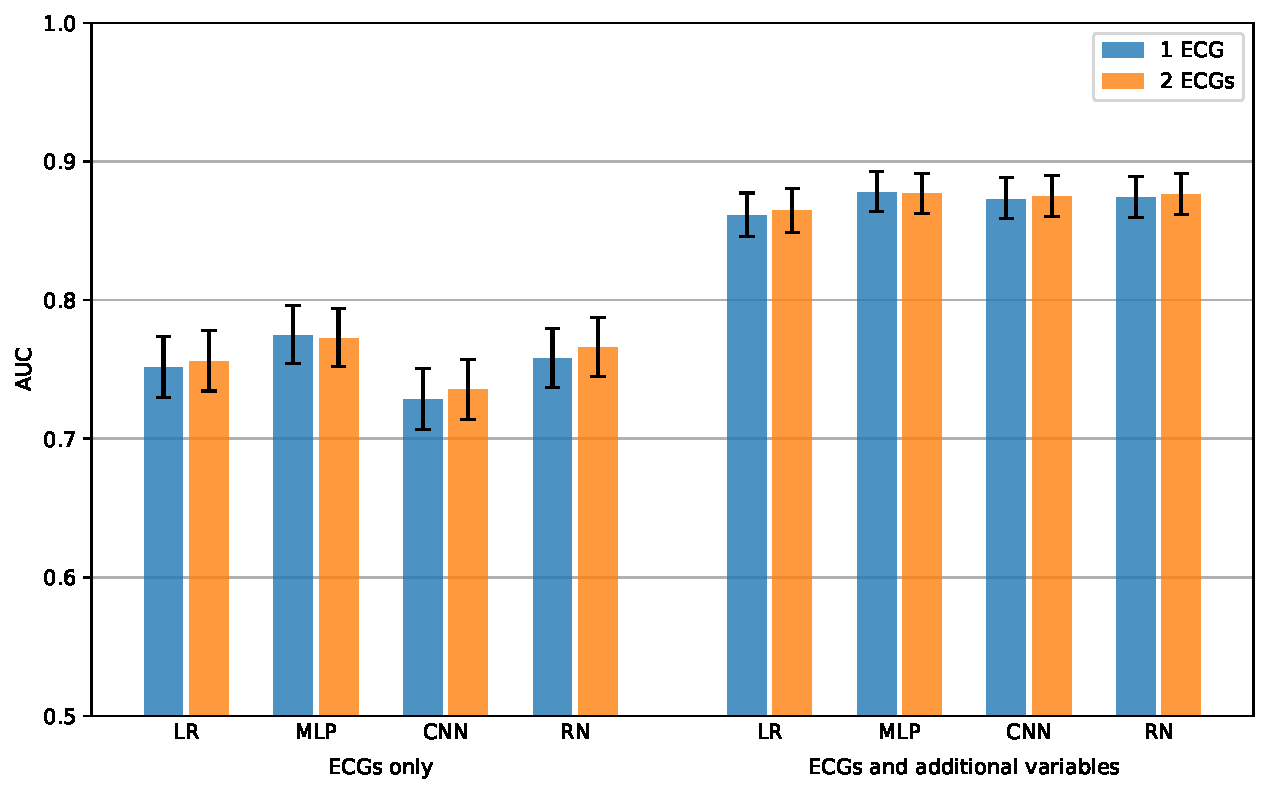
\includegraphics[scale=0.6]{main_results.pdf}
    \caption{Main results}
    \label{fig:mainresults}
\end{figure}

\subsection{Models with versus without additional clinical variables}
As can be seen in Figure 2a, all models improved considerably with the inclusion of additional clinical variables. Models using only the ECG had an AUC around 0.77 (95\% CI for the best model: 0.754-0.796), while those including the additional variables had an AUC around 0.87 (95\% CI for the best model: 0.864-0.893). The differences between models with and without a prior ECG were small in comparison. Of the four models, the MLP model performed the best, both with and without additional variables.

\subsection{Patients with versus without pathological index ECGs}
Figure \ref{fig:pathresults} shows the results stratified by the presence or absence of a pathological index ECG, for the models including additional variables. In general, all models performed slightly better in patients with non-pathological index ECGs, but there was no improvement by the addition of a prior ECG. Models based on only the ECG performed slightly better with an added prior ECG, but the best performing model (MLP) did not improve.

\begin{figure}[h!]
%    \centering
    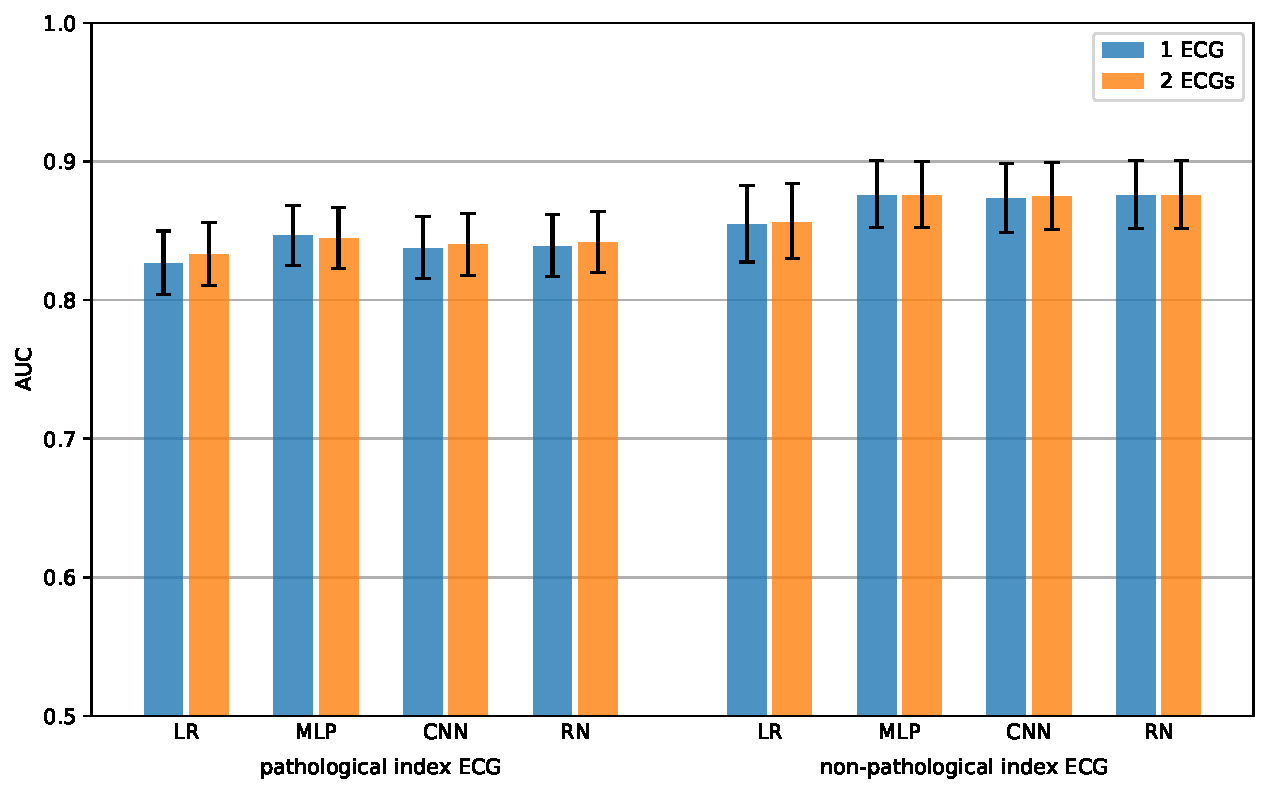
\includegraphics[scale=0.6]{path_results.pdf}
    \caption{Main results}
    \label{fig:pathresults}
\end{figure}

\subsection{Patients in different age groups}
The performance of the models in the different age groups are shown in the appendix. Among the models using ECG only, the best model (MLP) improved by the addition of a previous ECG in patients up to 64 years, while the performance declined in those aged 65-75 years, suggesting that a previous ECG does not make a big difference. Models using additional clinical variables performed substantially better in younger patients, with e.g. a mean AUC of 0.92 with the MLP model in those 18-50 years and 0.82 in those over 76 years. This pattern was not present in the models using ECG only.

\subsection{Patients with versus without previous AMI}
In patients with or without a previous AMI, adding a historic ECG generally did not improve the predictive ability of the models. The exception was the RN models using only ECG and the LR models with additional clinical variables, but both these models were outperformed by the corresponding MLPs. The AUC of all models, both with and without additional clinical variables, were substantially lower in patients with versus without a previous AMI. 

\subsection{MACE components as individual outcomes}
There were no meaningful predictive improvements with the addition of a previous ECG when evaluating the models on UA, AMI and death separately. For models based on ECG only, UA was harder to predict (best AUC 0.71) than AMI (best AUC 0.80) and 30-day mortality (AUC 0.83). The corresponding AUC for models including additional clinical variables were 0.77, 0.92 and 0.89. 

\section{Discussion}
This study aimed to determine whether the addition of a previous ECG would improve the AUC of ML models predicting MACE within 30 days in ED chest pain patients. The purpose was thus not to identify the best predictive model for this outcome, but rather to give "equal opportunity" for models with different inputs, to see which performed the best. Our results consistently showed no improvements from prior ECGs, across several different models, additional input features, and patient subgroups, including patients of different ages, with or without prior AMI, and with pathological or non-pathological index ECGs.

These findings are somewhat counterintuitive because they run against current guidelines and best practices for manual ECG analysis, with the implication that it might be a waste of time to consider prior ECGs. While one should be careful to draw hasty conclusions, it might be sensible to further scrutinize the evidence in favor of evaluating prior ECGs, especially when it is based on data that is several decades old.

The lack of model improvement from prior ECGs is an indication that future research on ML for predicting MACE might be better focused on adding variables other than prior ECGs to the models. This might turn out to be a good thing, since not all patients have prior ECGs, and not all health care environments have access to digital ECG databases, so to the extent that an ML model can maintain predictive performance absent prior ECGs, such models will have a wider applicability.

Our models consistently performed better for several subgroups (though not with respect to prior ECGs): patients with non-pathological index ECGs, younger patients, and those with no history of AMI, were all “easier” to predict than their counterparts. These patients are typically healthier and have fewer comorbidities, so one reason for the increased model performance could be that whenever there is no sign of MACE, such patients are more likely to in fact be healthy, and conversely, when there are signs of MACE, it counts for more because the signal is less likely to be "obscured" by comorbidities or other explanations.

Interestingly, the best models in our comparisons were not the most advanced – the MLP outperformed both the CNN and RN models despite markedly fewer trainable parameters. We speculate that this is because the MLP model used the Glasgow features, which are expert features known to be useful for ECG analysis, while the CNN and RN models learned everything from the raw signal. In this sense, the MLP models were “pre-trained” with human knowledge and the CNN models were not. Given enough data and computing power, we expect that the CNN and RN models can perform at least similar to the MLP models.

The MLP models used in this study are similar to that employed by Ohlsson et al.8 who combined Glasgow features from serial ECGs in a small neural network. When adding a previous ECG, AUC improved by three percentage points (0.85 to 0.88). In our study, we had almost three times more training data but were still unable to achieve a similar AUC, and we found no clinically significant improvement from a previous ECG. A possible explanation is that the patient populations were different; Ohlsson’s data were collected in 1990-1997 and ours in 2017-18. Indeed, our AMI prevalence was 7.4\% compared to over 20\% in the Ohlsson study. In addition, the characteristics of the AMI patients and the ECG findings are likely different due to new AMI definitions and highly sensitive troponin assays. 

Although we only tested four different ML models, our results suggest that ML models predicting MACE in ED chest pain patients do not improve significantly by the addition of a prior ECG, and that adding other information might be more beneficial. However, it should be noted that ED physicians may still make better decisions by comparing new and old ECGs. Humans do not assess the ECG in the same way as ML models, and ED physicians are often interested in additional outcomes other than MACE within 30 days.

\subsection{Limitations}
This study has some limitations. First, we used AUC as the metric for model performance whereas a fixed classification threshold would be used for decision-making in clinical care. We used AUC since the chosen threshold might differ in various clinical settings, and since the AUC reflects the overall performance at all thresholds. Although we cannot exclude it, we find it unlikely that the results would have been qualitatively different with a fixed classification threshold.

Second, as observed in the results section on patient characteristics, there were differences between the training, validation and test sets, particularly with respect to disease history. These differences likely occurred because the ESC-TROP database only includes the first visit for each patient during the study period, and because we split the dataset chronologically rather than randomly. The test set (and to a lesser degree the validation set) was therefore biased toward patients who rarely visit the ED with chest pain. The models’ performances may have been worse as a result, and it is possible that splitting the dataset randomly might have improved performance. However, since this applied similarly to models with and without a previous ECG, and because the proportion of MACE was similar across the splits, we find it reasonable to believe that the qualitative effects on the results were negligible. Furthermore, randomly splitting the data comes with its own set of drawbacks, which are avoided by a chronological split \citep{steyerberg2009}.

Third, our study does not include STEMI patients, so it is plausible, if not likely, that our results would differ for that patient group. However, STEMI patients, when detected, have a specific pathway through the health-care system, which largely bypasses the ED. In fact, if STEMI is detected, the patient will immediately be transferred to the cardiac care unit, so from the perspective of the ED physician, STEMI patients are "someone else's problem".

Fourth, the model selection is highly dependent on the search space of the hyper-parameters, the search algorithm used, and the available computational resources. In this study, the hyper-parameters for each model were determined separately for each set of inputs by randomly sampling the parameter space 400 times, with the exception of the pre-trained RN model that was only sampled 200 times, due to time constraints. It is possible that a different or more exhaustive search strategy would have yielded a different result, but again this would always be the case regardless of method, since the hyper-parameter space is infinite. We note that our results in the test and validation sets were similar, which indicates that we did not overfit on the training set. 

Finally, it is possible that the addition of a previous ECG would make a difference with more sophisticated models or feature engineering. However, we find it reasonable to believe that such differences would be small in magnitude and therefore of limited clinical significance, especially if clinical variables such as blood tests and comorbidities are included in the model.

\subsection{Conclusion}
In this study, we found no improvement by adding a prior ECG to ML models predicting MACE within 30 days in ED chest pain patients. Our results were consistent across model types, patient groups, and additional model inputs. These findings suggest that ML models predicting MACE will perform equally well for patients without prior ECGs, and in the many health care settings lacking a digital ECG database.

\section*{Declaration of competing interest}
The are no conflicts of interest to declare.
%% AB: Move appendix to separate file.

%% %% The Appendices part is started with the command \appendix;
%% %% appendix sections are then done as normal sections
%% \appendix

%% \section{Results with confidence intervals}
%% \label{sec:appendix:results}

%% \section{Definition of MACE}
%% \label{sec:appendix:mace}

%% \section{Excluded patients}
%% \label{sec:appendix:excluded}

%\section*{References}

\bibliography{serial_ecg_paper}

\end{document}
